\section{REST-API (J.L.)}
\label{sec-restapi}

Um die Daten, welche durch die Pipeline in die Datenbank geschrieben wurden, 
für das Web-Frontend verfügbar zu machen, wurde eine REST-API implementiert. 
Die REST-API wurde in Python \cite{python} mittels der Library FastAPI \cite{fastapi} 
programmiert. Dabei wurde die Library SQL-Alchemy \cite{sqlalchemy} als ORM-Tool 
zur Anbindung an die Datenbank verwendet.

\subsection{FastAPI}

FastAPI ist ein Framework zur schnellen Entwicklung von REST-APIs. 
Es ist ein Open-Source-Projekt. Als Gründe für die Wahl des Frameworks sind anzuführen: 

\subsubsection{Erfahrungen und Bekanntheit}
FastAPI ist ein bekanntes Framework, das in letzter Zeit zunehmend Bekanntheit erlangt 
hat und nun seine Position gegenüber anderen Frameworks wie z.B. Flask \cite{flask} und 
Django \cite{django} gefestigt hat. Da bereits Erfahrungen mit Flask und FastAPI bestehen 
lag die Wahl eines dieser Frameworks nahe. FastAPI hat sich nach eigenen Erfahrungen als 
einfacher in der Handhabung und performanter erwiesen.

\subsubsection{Parsen und Validieren}
FastAPI bietet das Parsen und Validieren von Daten aus Requests an. Dadurch kann 
auf manuell implementierte repetitive Überprüfungen verzichtet werden und es kann mit
einer grundlegenden Typsicherheit programmiert werden. Dies äußert sich auch in den Rückgaben,
die bei der Definition eines Rückgabeschemas diesem zu entsprechen haben. Des Weiteren bietet 
FastAPI einen einfacheren Zugriff auf Daten aus dem Request, da es über die definierten Keywords
den Zugriff auf Path- oder Query-Parameter sowie Inhalte aus dem Request-Body erleichtert.

\subsubsection{SwaggerUI und OpenAPI Konformität}
FastAPI generiert zu Dokumentationszwecken automatisch eine SwaggerUI \cite{swaggerui}, 
die einen Überblick über alle vorhandenen API Routen bietet. Dies ist im folgenden Screenshot der 
SwaggerUI zu sehen. Zudem können unter geringem Aufwand Definitionen der Rückgabewerte der 
einzelnen Routen erstellt werden, sodass FastAPI daraus eine OpenAPI-konforme \cite{openapi} 
openapi.json Datei generieren kann. Diese kann zur einfachen Anbindung an einen konsumierenden 
Service, so beispielsweise auch im Frontend, verwendet werden. Somit kann hier repetitiver und 
primitiver Programmieraufwand vermieden werden. ~\\
\begin{figure}[!htb]
 \centering
 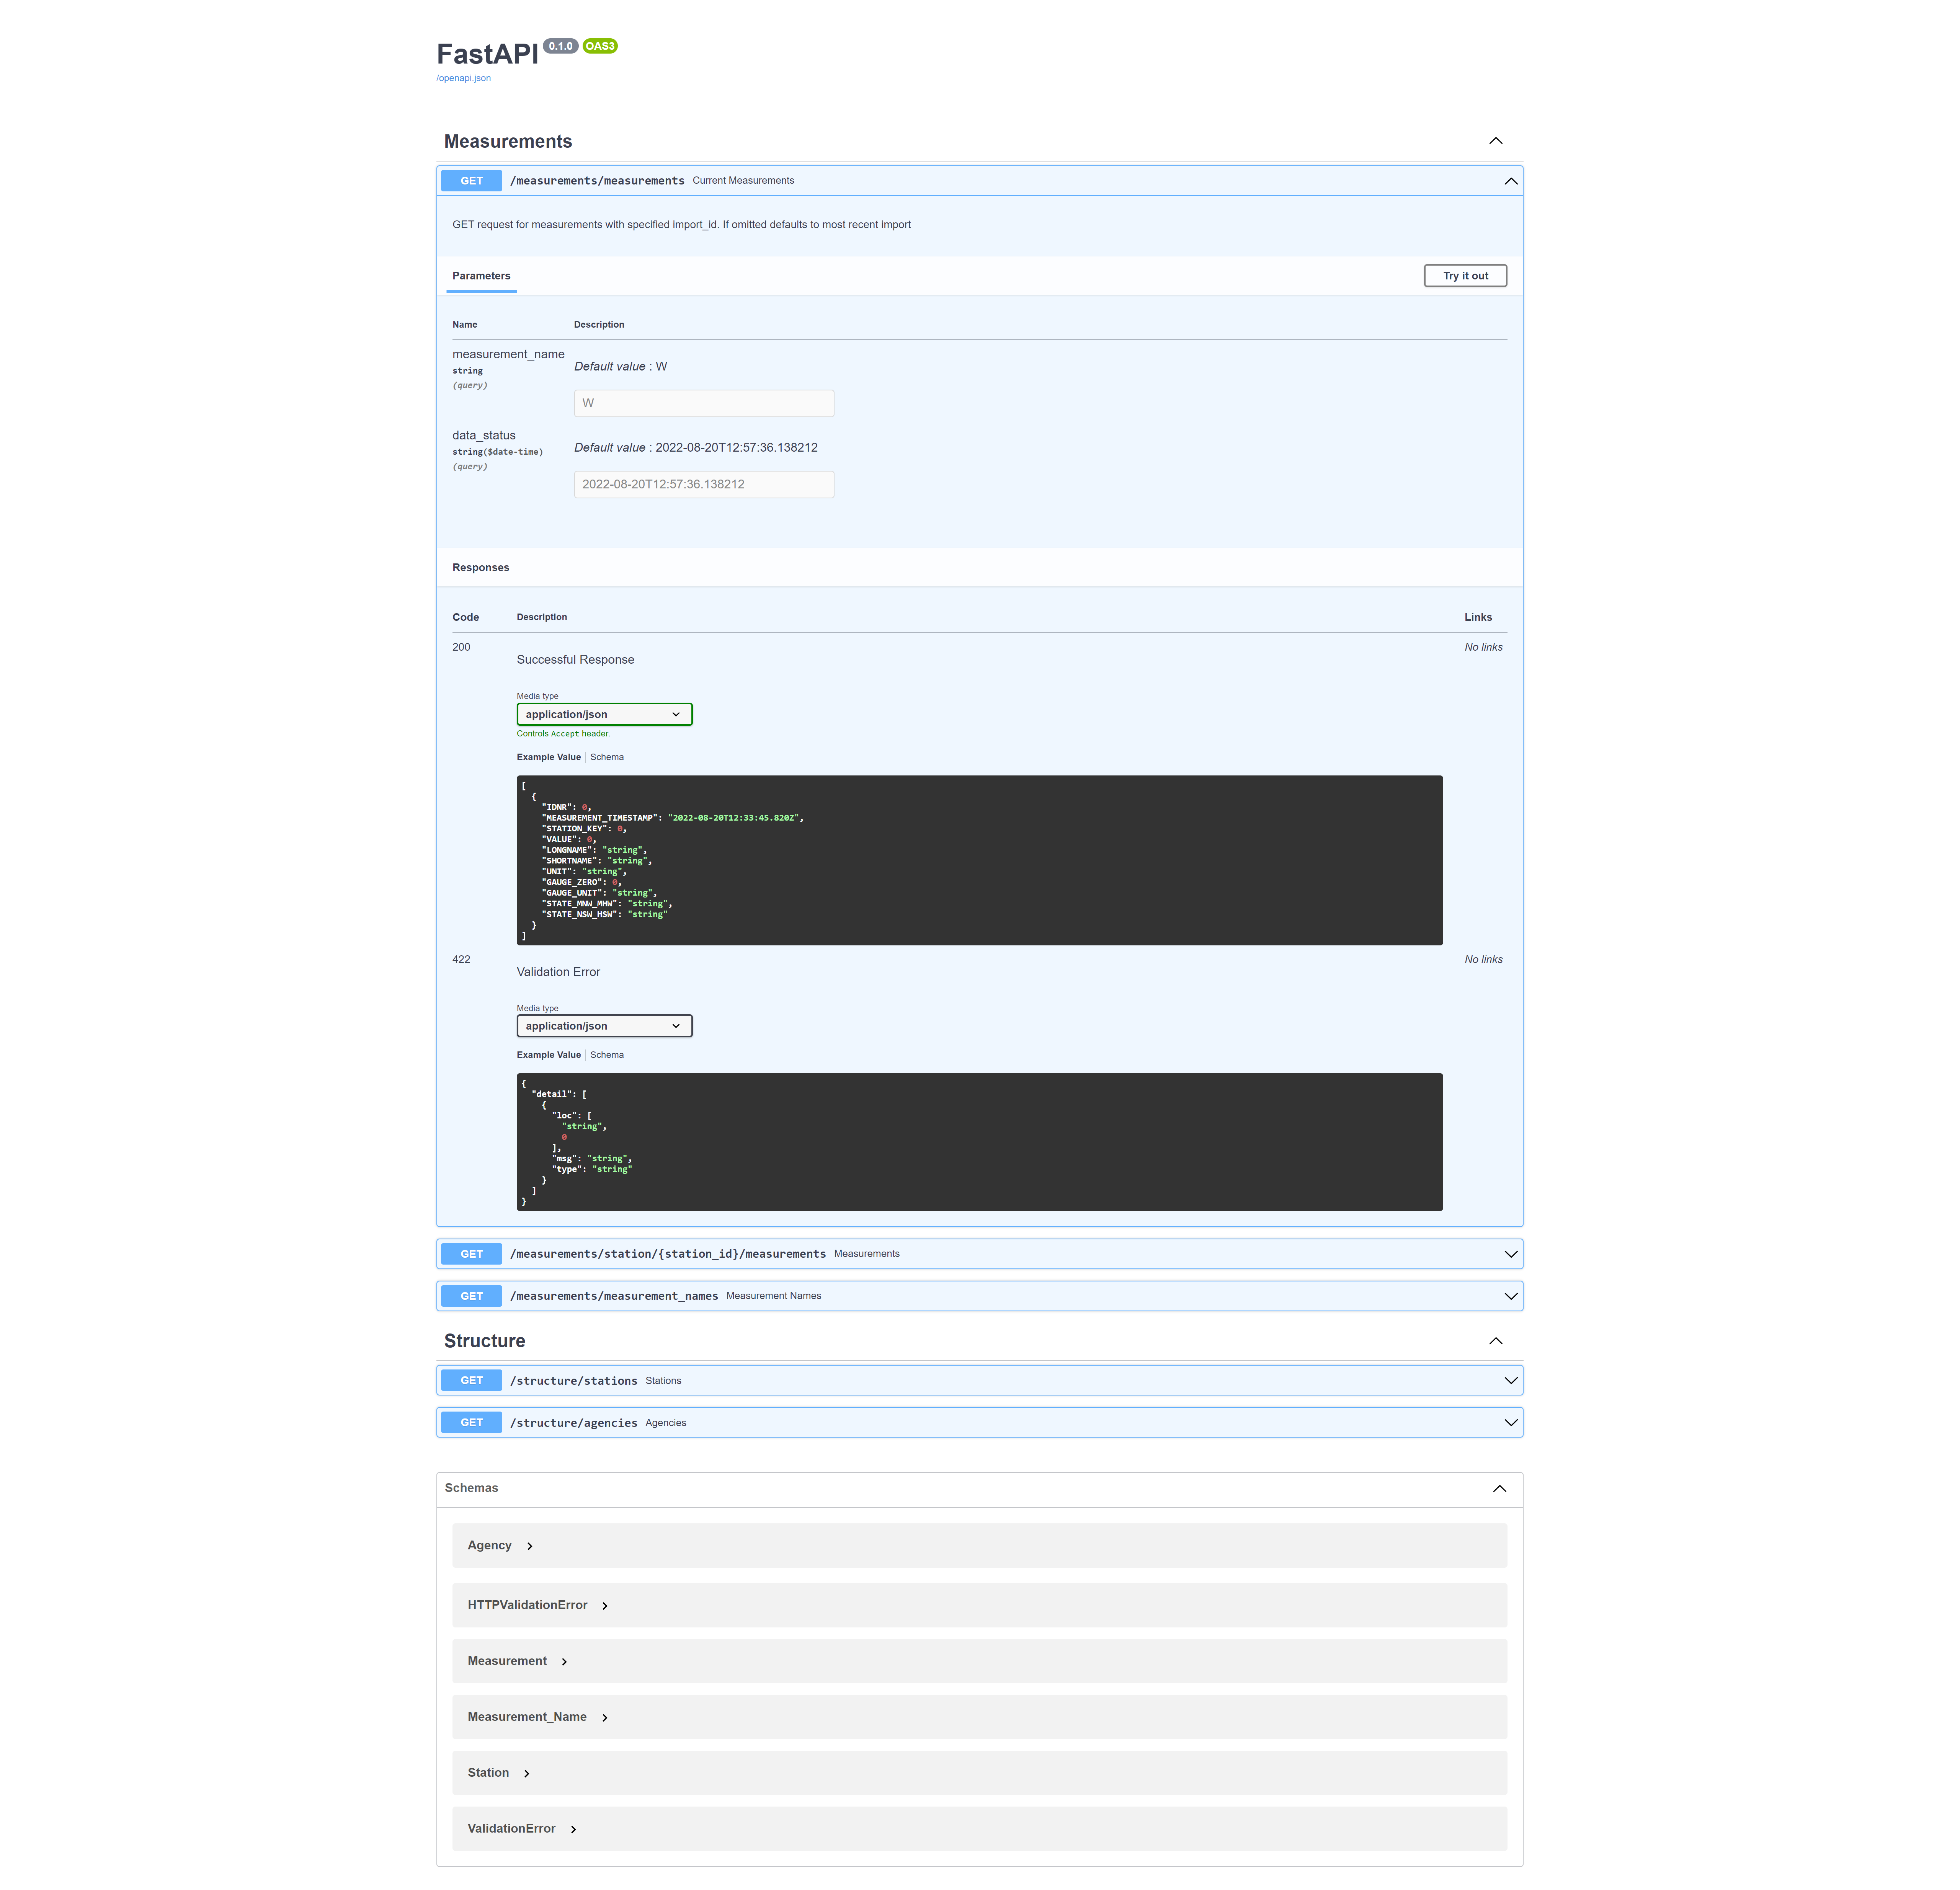
\includegraphics[width=\linewidth]{figures/SwaggerUI.png}
 \caption{Screenshot der SwaggerUI}
 \label{fig:SwaggerUI}
\end{figure}~\\
In diesem Screenshot ist die aus den Angaben automatisch generierte SwaggerUI zu sehen. 
Besonders hervorzuheben ist hier der ausgekplappte Request, der mögliche Antworten der 
API schemahaft darstellt.


\subsubsection{Strukturierbarkeit der API}
Die API kann mit sogenannten Routern in mehrere Teile strukturiert werden. 
Dadurch ist eine hohe Kohäsion gegeben, da logisch unterschiedliche Aufgaben getrennt behandelt 
werden können. Zugleich ist auch die Übersichtlichkeit und somit auch die Wartbarkeit erhöht, 
da die Strukturierung in Form von einer Aufteilung sowohl auf Datei-, als auch Routenebene 
sowie der Aufteilung in der SwaggerUI vorliegt.

\subsection{Aufbau der API}
Die API wurde in zwei Router eingeteilt. 
Routen, die mit dem Prefix /structure beginnen, liefern Informationen über die 
vorhandenen Stationen und über die vorhandenen Behörden. 
Routen, die mit dem Prefix /measurements beginnen, liefern Informationen über 
Messwerte zurück. Dieses Diagramm soll den grundlegenden Aufbau darstellen: ~\\

\begin{figure}[H]
    \centering
    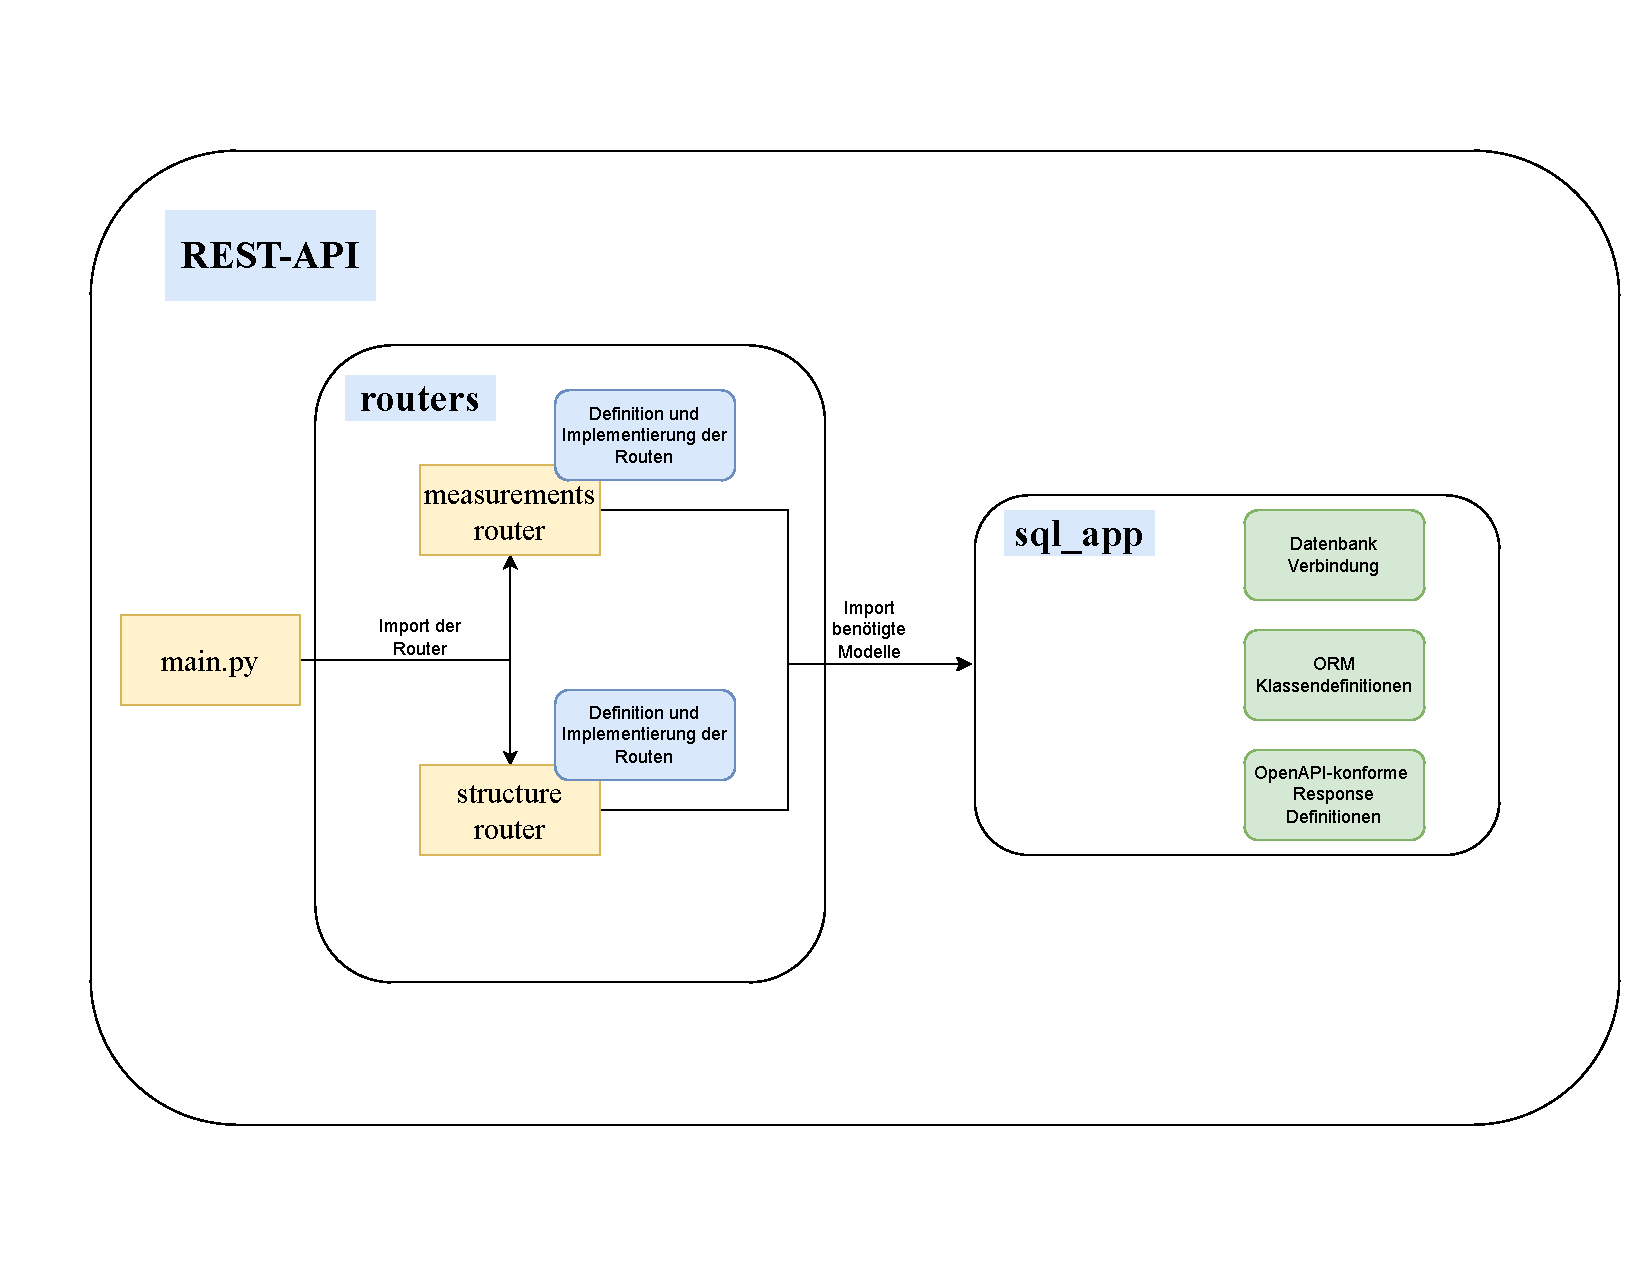
\includegraphics[width=\linewidth]{figures/REST-API-Aufbau.drawio.pdf}
    \caption{Diagram der REST-API}
    \label{fig:REST-API-Structure}
\end{figure}~\\
Im folgenden Code Auszug ist die main.py zu sehen, in der die grundlegende Struktur erstellt wird.~\\

\begin{lstlisting}[language={Python}, caption={Aufbau der API}, captionpos=b, label={fig:pythonAPI}]
    from fastapi import FastAPI
    from starlette.middleware.cors import CORSMiddleware
    from routers import measurements, structure
    from sql_app import models
    from sql_app.database import engine
    
    models.Base.metadata.create_all(bind=engine)
    app = FastAPI()
    app.include_router(measurements.router, 
        prefix="/measurements",tags=["Measurements"])
    app.include_router(structure.router, 
        prefix="/structure",tags=["Structure"])
    app.add_middleware(
        CORSMiddleware,
        allow_origins=["*"],
        allow_credentials=False,
        allow_methods=["*"],
        allow_headers=["*"],
    )
\end{lstlisting}~\\
Über die Methode \textit{app.include\_router()} wird ein sogenannter Router zur FastAPI Instanz 
hinzugefügt. 
Der Prefix bestimmt unter welchem Pfad die Routen aus dem hinzugefügten Router erreichbar sind. \\
Über die Methode \textit{app.add\_middleware()} wird hier erreicht, dass sämtlichen Antworten durch 
die API Header angefügt werden. Diese sorgen dafür, dass ein Aufrufen der API aus einem Webbrowser 
heraus (bspw. durch das Frontend) möglich ist und nicht zu Problemen aufgrund der 
CORS \cite{cors} Richtlinien führt. 

\subsection{Anbindung an die Datenbank}

Zum Abfragen von Daten aus der Datenbank wurde SQL-Alchemy verwendet. 
SQL-Alchemy ist ein ORM-Tool zum Abfragen und Manipulieren von Daten aus einer SQL-Datenbank. 
Mit dem folgenden Ausschnitt aus dem Quellcode wird eine Klasse erstellt, die eine Tabelle 
der Datenbank repräsentiert. Dies stellt am Anfang einen Overhead dar, da die zu verwendenden 
Tabellen, einschließlich ihrer Spalten vorab definiert werden müssen. Jedoch ergibt sich 
durch das Definieren dieser Klasse eine höherere Wiederverwendbarkeit und eine typsichere Verwendung 
von Daten aus der Datenbank gegenüber Alternativen, die auf SQL-Statements in Form von Strings und 
Rückgaben in Form von Listen basieren. Abfragen an die Datenbanken können somit auch sehr 
einfach und schnell erstellt werden. ~\\

\begin{lstlisting}[language={Python}, caption={Anbindung an die Datenbank}, captionpos=b, label={fig:pythonDBModels}]
from sqlalchemy import Column, Integer, String
from .database import Base

class Measurement_Name(Base):
    __tablename__ = "TBL_MEASUREMENT_NAME"
    
    IDNR = Column(Integer, primary_key=True)
    LONGNAME = Column(String)
    SHORTNAME = Column(String)
\end{lstlisting}~\\
Mittels der oben definierten Klasse kann auf sehr simple Weise für eine Route eine 
Abfrage erstellt werden. Siehe dazu folgendes Beispiel: ~\\

\begin{lstlisting}[language={Python}, caption={Anbindung an die Datenbank}, captionpos=b, label={fig:SQL-ALchemy Query}]
@router.get("/measurement_names", response_model=
    list[response_models.Measurement_Name])
def measurement_names(
db: Session = Depends(get_db)):
    return db.query(models.Measurement_Name
    ).with_entities(
        models.Measurement_Name.SHORTNAME,
        models.Measurement_Name.LONGNAME
    ).all()
\end{lstlisting}~\\
Die oben gezeigte Abfrage mittels SQL-Alchemy resultiert in einer SQL-Abfrage 
äquivalent zu der folgenden PostgreSQL-Abfrage~\\

\begin{lstlisting}[language={SQL}, caption={Äquivalente SQL Abfrage}, captionpos=b, label={fig:pythonDBModels}]
SELECT "SHORTNAME", "LONGNAME"
FROM "TBL_MEASUREMENT_NAME"
\end{lstlisting}~\\ 
Durch das Verwenden von SQL-Alchemy vereinfacht sich die Erstellung von Rückgaben, 
da die gefundenen Daten aus der Datenbank über das Key-Value Prinzip adressiert werden können 
und automatisch sämtliche Datentypen JSON-konform transformiert werden, bevor sie als 
Response von der API dem Client zurückgesendet werden. Dadurch wird primitiver und 
oft fehlerbehafteter Programmieraufwand vermieden, indem u.a. Datumswerte in ihre 
ISO-DateString \cite{iso-datestring} Repräsentation überführt werden.

\subsection{OpenAPI-Konformität der API}
OpenAPI \cite{openapi} ist ein Standard zur Beschreibung einer HTTP-API, der sowohl für 
Menschen als auch Computer verständlich ist. Der Standard beschreibt die verfügbaren Routen, 
die erwarteten Input-Daten durch den Client und die zu erwartende Response einschließlich 
eventueller Datentypen. Der Standard ist unabhängig von der Programmiersprache. Durch die 
Verwendung des Standards können ansprechende Weboberflächen zur Exploration der Möglichkeiten 
der API, beispielsweise in Form einer SwaggerUI generiert werden. Ferner kann durch ein 
geeignetes Tool Quellcode generiert werden, der Methoden, welche Daten aus der API abfragen können, 
sowie die Typdefinitionen gemäß des Standards umfasst. Dadurch konnte im Frontend ein 
beträchtlicher Programmieraufwand vermieden werden. Die Typdefinition von JSON-Responses 
durch die API erfolgte nur einmal in der REST-API und konnte im Frontend gemäß der äquivalenten 
Datentypen verwendet werden. Siehe hierzu folgendes Beispiel für die Definition der Klasse 
Measurement\_Name, die als response\_model für die oben gezeigte API-Route verwendet wird. ~\\

\begin{lstlisting}[language={Python}, caption={Response Model Measurement\_Name}, captionpos=b, label={fig:Response Model}]
from pydantic import BaseModel
class Measurement_Name(BaseModel):
    SHORTNAME: str
    LONGNAME: str
\end{lstlisting}~\\